\hypertarget{colonel-bogey-march}{%
\section{Colonel Bogey March}\label{colonel-bogey-march}}

\begin{figure}[!ht]
  \begin{adjustwidth}{-\oddsidemargin-1in}{-\rightmargin}
    \centering
    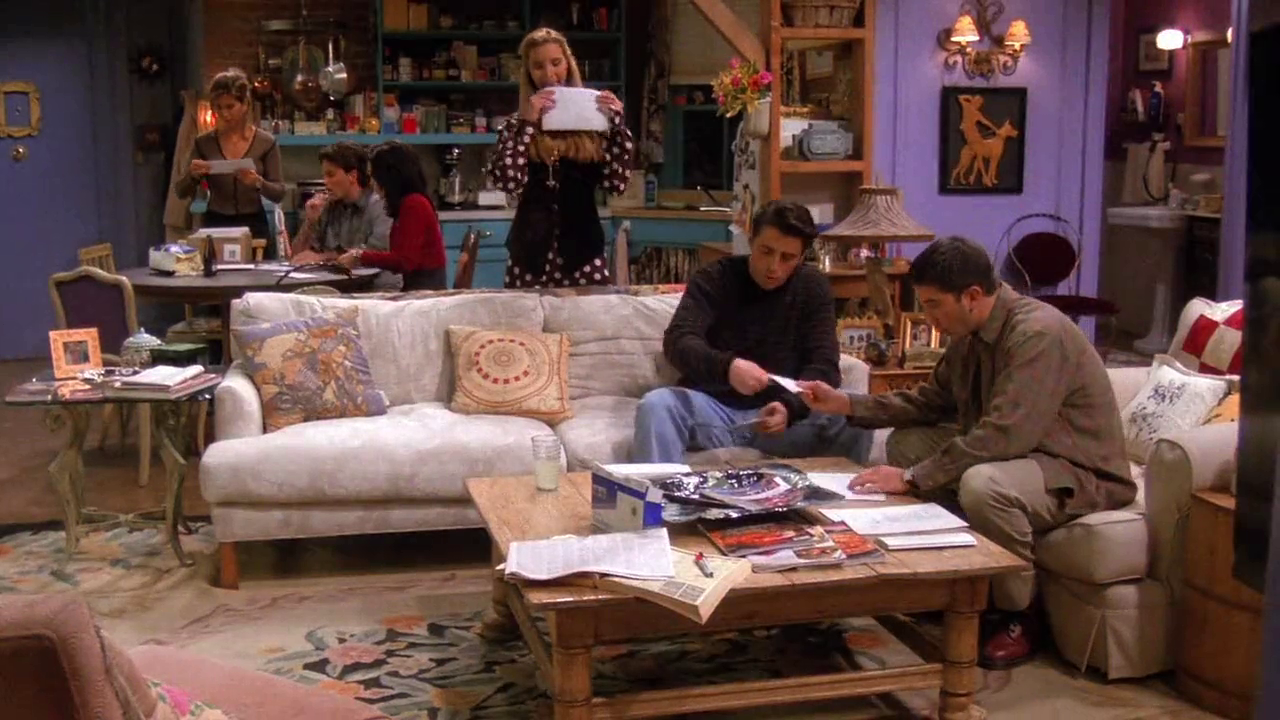
\includegraphics[trim={0 8cm 0 1cm,}, clip, width=\paperwidth]{./S01/img/18/colonel-bogey-march.png}
    % \caption{Colonel Bogey March\label{fig:colonel-bogey-march}}
  \end{adjustwidth}
\end{figure}

Ajudando Rachel com o envio de seu currículo, os amigos assobiam a
melodia \emph{Colonel Bogey March} (1914), composta pelo diretor de
música da \emph{Marinha Real de Plymouth}, o tenente inglês
\emph{Frederick Joseph Ricketts} (1881-1945).

Ela também foi usada no filme \emph{The Bridge on the River Kwai}
(1957), e pode ser ouvida em sua trilha sonora. O compositor
\emph{Malcolm Arnold} (1921-2006) ainda criaria uma contra-marcha
chamada \emph{River Kwai March}, que faz o acompanhamento de uma banda
de música com o assobio.

\hypertarget{referuxeancias}{%
\subsection{Referências}\label{referuxeancias}}

\begin{itemize}
\tightlist
\item
  \sloppy Minor British Institutions: Colonel Bogey - Independent (Inglês). \url{https://www.independent.co.uk/news/uk/this-britain/minor-british-institutions-colonel-bogey-2080160.html}
\item
  \sloppy The Bridge On The River Kwai (Soundtrack) - YouTube. \url{https://music.youtube.com/playlist?list=OLAK5uy_mfzGk0bXhekFyvLnYSMtJw-AX61a9dpHQ}
\end{itemize}

\hypertarget{popular-mechanics}{%
\section{Popular Mechanics}\label{popular-mechanics}}

\begin{figure}[!ht]
  \begin{adjustwidth}{-\oddsidemargin-1in}{-\rightmargin}
    \centering
    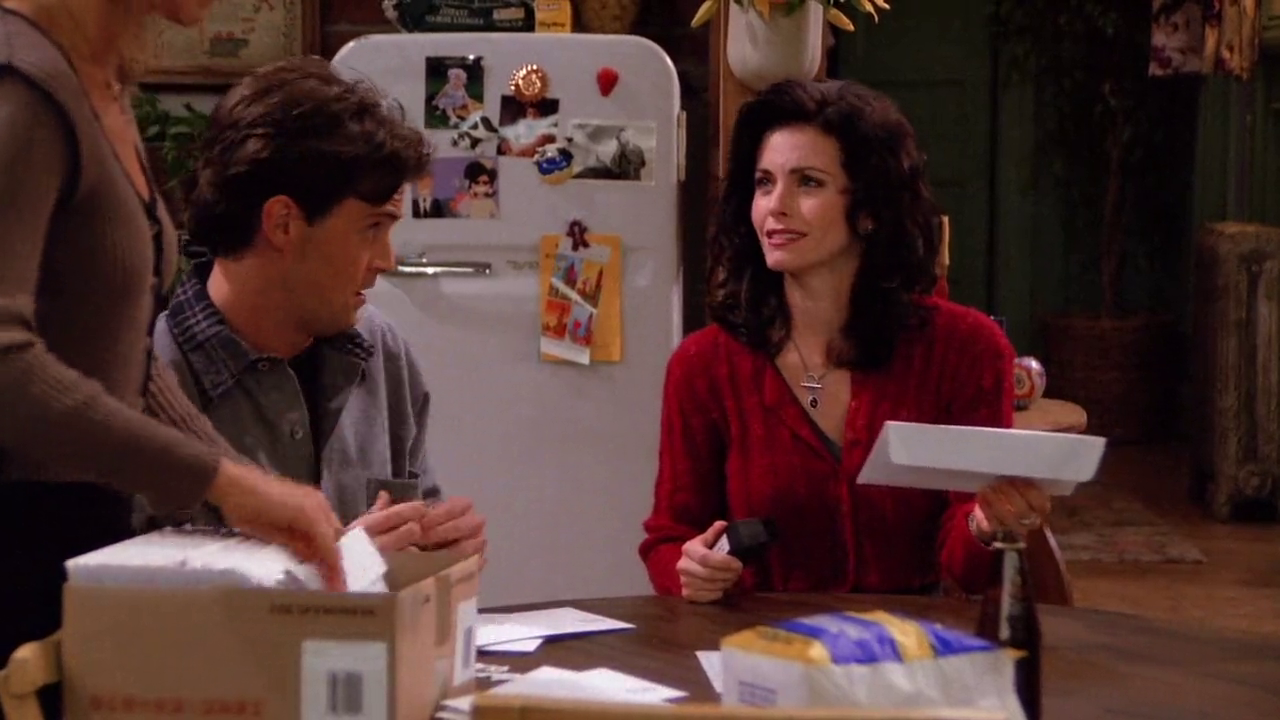
\includegraphics[trim={0 7cm 0 1cm,}, clip, width=\paperwidth]{./S01/img/18/popular-mechanics.png}
    % \caption{Popular Mechanics\label{fig:popular-mechanics}}
  \end{adjustwidth}
\end{figure}

\begin{tcolorbox}[enhanced,center upper,
    drop fuzzy shadow southeast, boxrule=0.3pt,
    lower separated=false, breakable,
    colframe=black!30!dialogoBorder,colback=white]
\begin{minipage}[c]{0.16\linewidth}
  \raisebox{\dimexpr-\height+\ht\strutbox\relax}{
    \centering 
\includegraphics[width=1.4cm]{./assets/img/monica.png}
  }
   & \centering \scriptsize{Monica}
\end{minipage}
\hfill
\begin{minipage}[c]{0.8\linewidth}
  \textbf{- Do you really want a job with Popular Mechanics?}\\
  - Quer mesmo trabalhar com a Popular Mechanics?
\end{minipage}

\medskip
\begin{minipage}[c]{0.16\linewidth}
  \raisebox{\dimexpr-\height+\ht\strutbox\relax}{
    \centering 
\includegraphics[width=1.4cm]{./assets/img/chandler.png}
  }
   & \centering \scriptsize{Chandler}
\end{minipage}
\hfill
\begin{minipage}[c]{0.8\linewidth}
  \textbf{- Well, if you're gonna work for mechanics, those are the ones to work for.}\\
  - Se quer trabalhar com mecânicos, é com esses que você deve trabalhar.
\end{minipage}
\end{tcolorbox}

Monica se espanta que Rachel queira trabalhar com a \emph{Popular
Mechanics} (1902), revista especializada em trazer as últimas novidades
no mundo da tecnologia, ciência e indústria automotiva.

Chandler brinca com a palavra \emph{mechanics} e seu gênero indefinido.
Assim \emph{Mecânicas Polulares} podem ser tornar \emph{mecânicos
populares} (atentem as iniciais dos termos), e é para esses que ele acha
que ela deve trabalhar.

\begin{figure}
  \centering
  \begin{tikzpicture}
    \node [inner sep=0pt] at (0,0) {
      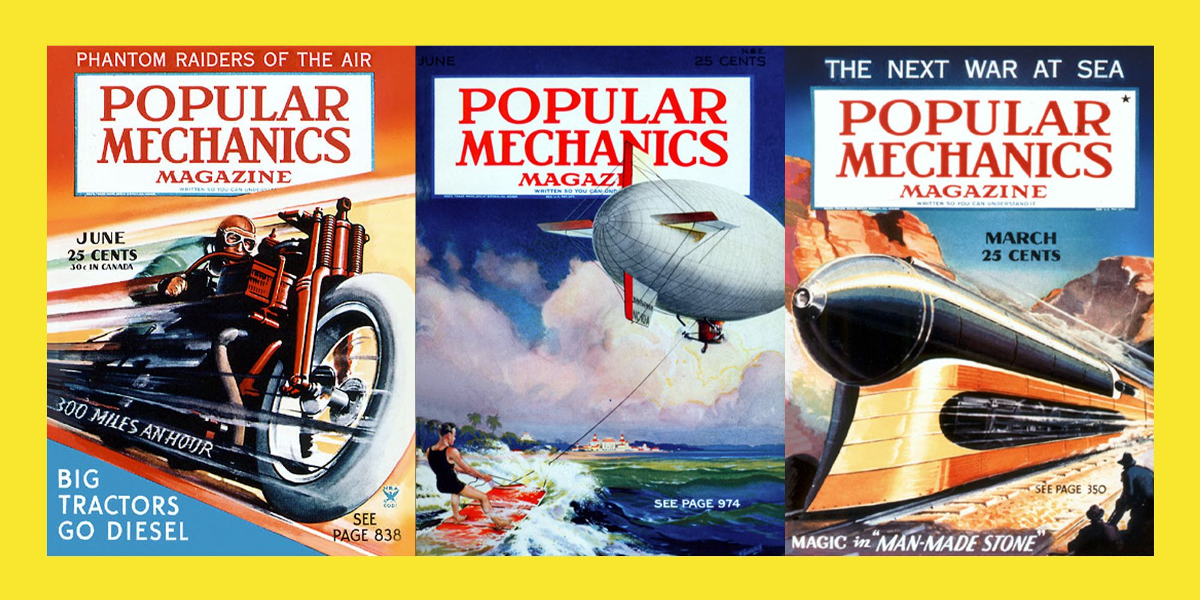
\includegraphics[width=0.8\textwidth,keepaspectratio]{./S01/img/18/popular-mechanics-covers.jpg}
    };
    \draw [white, rounded corners=\ClipSep, line width=\ClipSep]
    (current bounding box.north west) --
    (current bounding box.north east) --
    (current bounding box.south east) --
    (current bounding box.south west) -- cycle
    ;
    \end{tikzpicture}
    \caption{Popular Mechanics - Capas\label{fig:popular-mechanics-capas}}
\end{figure}

\hypertarget{referuxeancias-1}{%
\subsection{Referências}\label{referuxeancias-1}}

\begin{itemize}
\tightlist
\item
  \sloppy Site oficial (Inglês). \url{https://www.popularmechanics.com/about/a45/about-us/}
\end{itemize}

\hypertarget{flintstones}{%
\section{Flintstones}\label{flintstones}}

\begin{figure}[!ht]
  \begin{adjustwidth}{-\oddsidemargin-1in}{-\rightmargin}
    \centering
    
\includegraphics[trim={0 7cm 0 1cm,}, clip, width=\paperwidth]{./S01/img/18/flintstones.png}
    % \caption{Flintstones\label{fig:flintstones}}
  \end{adjustwidth}
\end{figure}

\begin{tcolorbox}[enhanced,center upper,
    drop fuzzy shadow southeast, boxrule=0.3pt,
    lower separated=false, breakable,
    colframe=black!30!dialogoBorder,colback=white]
\begin{minipage}[c]{0.16\linewidth}
  \raisebox{\dimexpr-\height+\ht\strutbox\relax}{
    \centering 
\includegraphics[width=1.4cm]{./assets/img/chandler.png}
  }
   & \centering \scriptsize{Chandler}
\end{minipage}
\hfill
\begin{minipage}[c]{0.8\linewidth}
  \textbf{- Is this still about her whole The 'Flintstones could have really happened' thing?}\\
  - Isso é porque ela disse 'A história dos Flintstones poderia ter acontecido'?
\end{minipage}
\end{tcolorbox}

Chandler menciona que um dos encontros de Ross havia dito que a história
dos \emph{Flintstones} (1960-1966) poderia ter acontecido. Para um
paleontólogo ouvir isso deve ser realmente frustante, visto que a
história, produzida pela \emph{Hanna-Barbera}, mostra a vida da família
\emph{Flintstone} que vive na idade da pedra, mas que convive com
dinosauros.

\begin{figure}
  \centering
  \begin{tikzpicture}
    \node [inner sep=0pt] at (0,0) {
      
\includegraphics[width=0.8\textwidth,keepaspectratio]{./S01/img/18/flintstones-personagens.jpg}
    };
    \draw [white, rounded corners=\ClipSep, line width=\ClipSep]
    (current bounding box.north west) --
    (current bounding box.north east) --
    (current bounding box.south east) --
    (current bounding box.south west) -- cycle
    ;
    \end{tikzpicture}
    \caption{Flintstones - Personagens\label{fig:flintstones-personagens}}
\end{figure}

\hypertarget{referuxeancias-2}{%
\subsection{Referências}\label{referuxeancias-2}}

\begin{itemize}
\tightlist
\item
  \sloppy Fandom Wiki (Inglês). \url{https://flintstones.fandom.com/wiki/The_Flintstones_(TV_series)}
\end{itemize}

\hypertarget{dee}{%
\section{Dee}\label{dee}}

\begin{figure}[!ht]
  \begin{adjustwidth}{-\oddsidemargin-1in}{-\rightmargin}
    \centering
    
\includegraphics[trim={0 6cm 0 2cm,}, clip, width=\paperwidth]{./S01/img/18/dee.png}
    % \caption{Dee\label{fig:dee}}
  \end{adjustwidth}
\end{figure}

\begin{tcolorbox}[enhanced,center upper,
    drop fuzzy shadow southeast, boxrule=0.3pt,
    lower separated=false, breakable,
    colframe=black!30!dialogoBorder,colback=white]
\begin{minipage}[c]{0.16\linewidth}
  \raisebox{\dimexpr-\height+\ht\strutbox\relax}{
    \centering 
\includegraphics[width=1.4cm]{./assets/img/chandler.png}
  }
   & \centering \scriptsize{Chandler}
\end{minipage}
\hfill
\begin{minipage}[c]{0.8\linewidth}
  \textbf{- Could you want her more?}\\
  - Poderia estar mais apaixonado?
\end{minipage}

\medskip
\begin{minipage}[c]{0.16\linewidth}
  \raisebox{\dimexpr-\height+\ht\strutbox\relax}{
    \centering 
\includegraphics[width=1.4cm]{./assets/img/ross.png}
  }
   & \centering \scriptsize{Ross}
\end{minipage}
\hfill
\begin{minipage}[c]{0.8\linewidth}
  \textbf{- Who?}\\
  - Por quem?
\end{minipage}

\medskip
\begin{minipage}[c]{0.16\linewidth}
  \raisebox{\dimexpr-\height+\ht\strutbox\relax}{
    \centering 
\includegraphics[width=1.4cm]{./assets/img/chandler.png}
  }
   & \centering \scriptsize{Chandler}
\end{minipage}
\hfill
\begin{minipage}[c]{0.8\linewidth}
  \textbf{- Who? Dee, the sarcastic sister from What's Happening!!}\\
  - Por quem? Dee, a irmã sarcástica de What's Happening!!
\end{minipage}
\end{tcolorbox}

Ross tenta disfarçar sua paixão por Rachel, mas Chandler logo se toca e
tenta fazer com que ele admita. Ele menciona \emph{Dee}, personagem da
\emph{sitcom} americana \emph{What's Happening!!} (1976-1979). \emph{Dee
Thomas} é irmã mais nova de \emph{Raj}, protagonista da série.

\begin{figure}
  \centering
  \begin{tikzpicture}
    \node [inner sep=0pt] at (0,0) {
      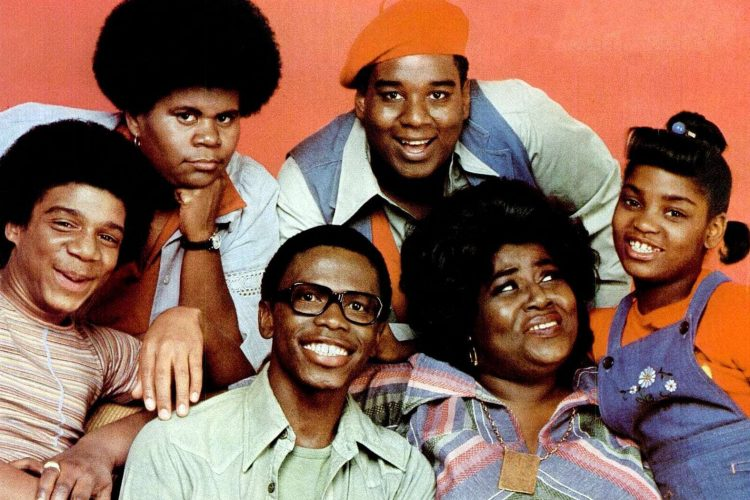
\includegraphics[width=0.8\textwidth,keepaspectratio]{./S01/img/18/whats-happening.jpg}
    };
    \draw [white, rounded corners=\ClipSep, line width=\ClipSep]
    (current bounding box.north west) --
    (current bounding box.north east) --
    (current bounding box.south east) --
    (current bounding box.south west) -- cycle
    ;
    \end{tikzpicture}
    \caption{What’s Happening - Personagens\label{fig:what-s-happening-personagens}}
\end{figure}

\hypertarget{referuxeancias-3}{%
\subsection{Referências}\label{referuxeancias-3}}

\begin{itemize}
\tightlist
\item
  \sloppy Wikipédia. \url{https://en.wikipedia.org/wiki/What%27s_Happening!!}
\end{itemize}

\hypertarget{the-jamestown-colony-of-virginia}{%
\section{The Jamestown colony of
Virginia}\label{the-jamestown-colony-of-virginia}}

\begin{figure}[!ht]
  \begin{adjustwidth}{-\oddsidemargin-1in}{-\rightmargin}
    \centering
    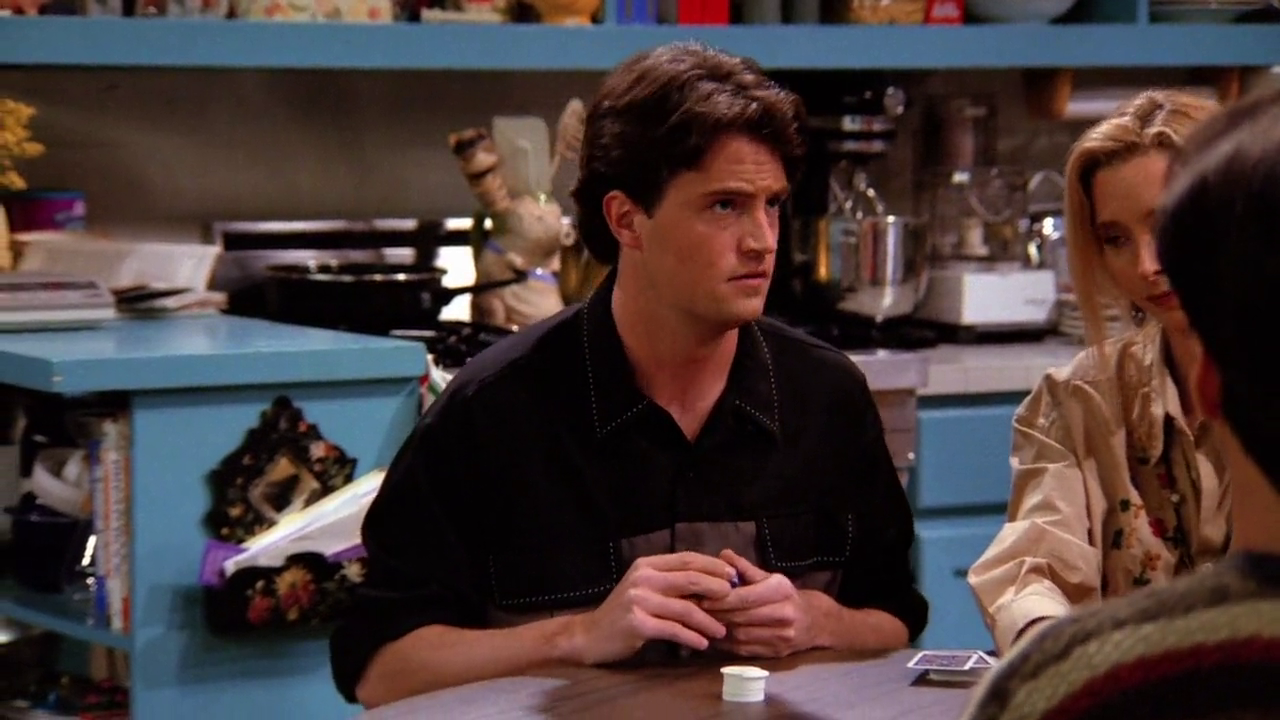
\includegraphics[trim={0 7cm 0 1cm,}, clip, width=\paperwidth]{./S01/img/18/the-jamestown-colony-of-virginia.png}
    % \caption{The Jamestown colony of Virginia\label{fig:the-jamestown-colony-of-virginia}}
  \end{adjustwidth}
\end{figure}

\begin{tcolorbox}[enhanced,center upper,
    drop fuzzy shadow southeast, boxrule=0.3pt,
    lower separated=false, breakable,
    colframe=black!30!dialogoBorder,colback=white]
\begin{minipage}[c]{0.16\linewidth}
  \raisebox{\dimexpr-\height+\ht\strutbox\relax}{
    \centering 
\includegraphics[width=1.4cm]{./assets/img/ross.png}
  }
   & \centering \scriptsize{Ross}
\end{minipage}
\hfill
\begin{minipage}[c]{0.8\linewidth}
  \textbf{- Rach, we've got to settle.}\\
  - Rach, vamos se acertar.
\end{minipage}

\medskip
\begin{minipage}[c]{0.16\linewidth}
  \raisebox{\dimexpr-\height+\ht\strutbox\relax}{
    \centering 
\includegraphics[width=1.4cm]{./assets/img/rachel.png}
  }
   & \centering \scriptsize{Rachel}
\end{minipage}
\hfill
\begin{minipage}[c]{0.8\linewidth}
  \textbf{- Settle what?}\\
  - 'Assentar' o quê?
\end{minipage}

\medskip
\begin{minipage}[c]{0.16\linewidth}
  \raisebox{\dimexpr-\height+\ht\strutbox\relax}{
    \centering 
\includegraphics[width=1.4cm]{./assets/img/chandler.png}
  }
   & \centering \scriptsize{Chandler}
\end{minipage}
\hfill
\begin{minipage}[c]{0.8\linewidth}
  \textbf{- The Jamestown colony of Virginia.}\\
  - A colônia de Jamestown da Virginia.
\end{minipage}
\end{tcolorbox}

Tomada a devida liberdade com a tradução, Chandler faz um trocadilho com
a palavra \emph{settle}, que pode ter o sentido de pagamento ou de
colonização. Daí sua referência à \emph{The Jamestown colony of
Virginia} (1607), onde um grupo de aproximadamente 100 colonos fundaram
o primeiro assentamento da América do Norte, às margens do \emph{Rio
James}. A Companhia \emph{Virginia}, como ficou conhecido o grupo,
planejava buscar depósitos de ouro e prata no \emph{Novo Mundo}.

Na fala seguinte, Chandler diz que o \emph{Rei George} os deu a terra,
mas na verdade quem o fez foi o \emph{Rei James I}.

\hypertarget{referuxeancias-4}{%
\subsection{Referências}\label{referuxeancias-4}}

\begin{itemize}
\tightlist
\item
  \sloppy History (Inglês). \url{https://www.history.com/topics/colonial-america/jamestown}
\end{itemize}

\hypertarget{ya-yas-from-ikea}{%
\section{Ya-ya's from Ikea}\label{ya-yas-from-ikea}}

\begin{figure}[!ht]
  \begin{adjustwidth}{-\oddsidemargin-1in}{-\rightmargin}
    \centering
    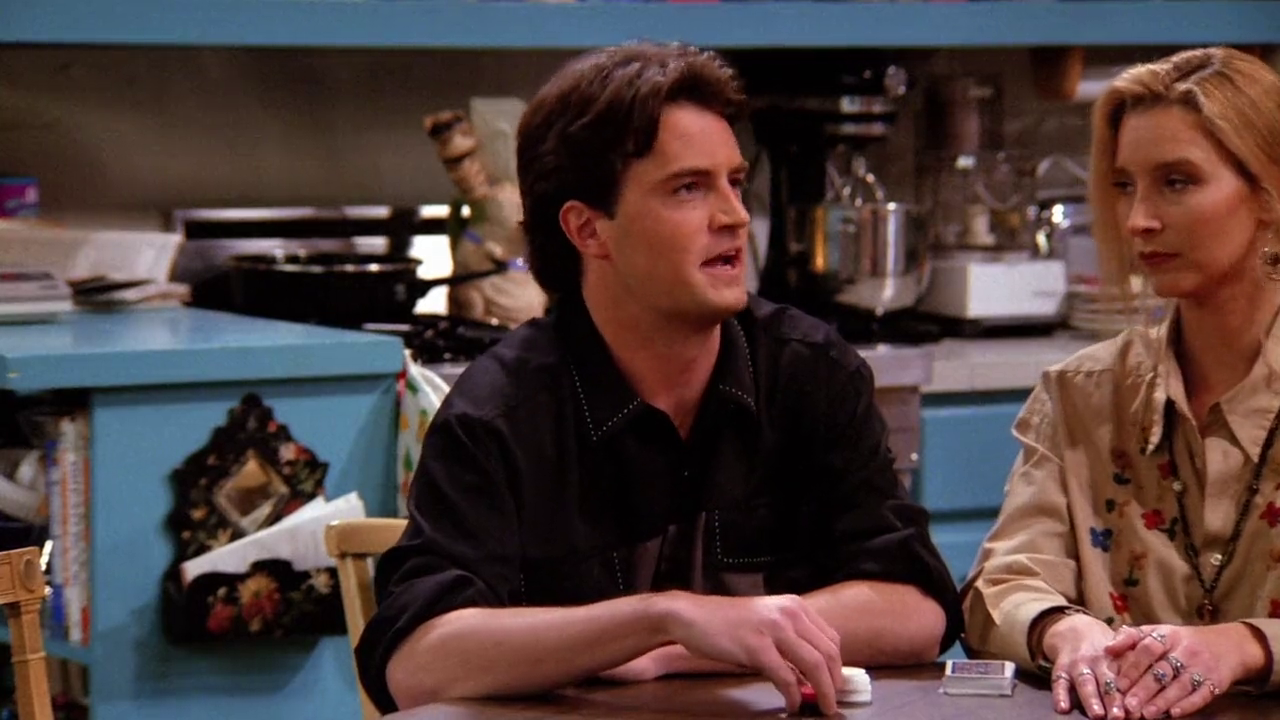
\includegraphics[trim={0 7cm 0 1cm,}, clip, width=\paperwidth]{./S01/img/18/ya-ya-s-from-ikea.png}
    % \caption{Ya-ya’s from Ikea\label{fig:ya-ya-s-from-ikea}}
  \end{adjustwidth}
\end{figure}

\begin{tcolorbox}[enhanced,center upper,
    drop fuzzy shadow southeast, boxrule=0.3pt,
    lower separated=false, breakable,
    colframe=black!30!dialogoBorder,colback=white]
\begin{minipage}[c]{0.16\linewidth}
  \raisebox{\dimexpr-\height+\ht\strutbox\relax}{
    \centering 
\includegraphics[width=1.4cm]{./assets/img/rachel.png}
  }
   & \centering \scriptsize{Rachel}
\end{minipage}
\hfill
\begin{minipage}[c]{0.8\linewidth}
  \textbf{- So, basically, you get your ya-yas by taking money from all of your friends.}\\
  - Basicamente, você obtém divertimento tomando dinheiro dos seus amigos.
\end{minipage}

\medskip
\begin{minipage}[c]{0.16\linewidth}
  \raisebox{\dimexpr-\height+\ht\strutbox\relax}{
    \centering 
\includegraphics[width=1.4cm]{./assets/img/ross.png}
  }
   & \centering \scriptsize{Ross}
\end{minipage}
\hfill
\begin{minipage}[c]{0.8\linewidth}
  \textbf{- Yeah.}\\
  - Pois é.
\end{minipage}

\medskip
\begin{minipage}[c]{0.16\linewidth}
  \raisebox{\dimexpr-\height+\ht\strutbox\relax}{
    \centering 
\includegraphics[width=1.4cm]{./assets/img/chandler.png}
  }
   & \centering \scriptsize{Chandler}
\end{minipage}
\hfill
\begin{minipage}[c]{0.8\linewidth}
  \textbf{- Yes, and I get my ya-yas from Ikea. You have to put them together yourself, but they cost a little less.}\\
  - Sim, e eu obtenho meu divertimento da Ikea. Você mesmo tem que montar, mas custa um pouco menos.
\end{minipage}
\end{tcolorbox}

Rachel usa a expressão \emph{get your ya-yas}, como uma forma de dizer
que Ross se diverte com a desgraça dos outros. Chandler, então, usa a
expressão \emph{ya-yas} e se refere a \emph{Ikea} (1943), empresa de
mobiliário e decoração de baixo custo para casas, em que os clientes
montam os próprios móveis. A expressão \emph{ya-yas} soa como uma
palavra sueca, e ele tira proveito disso já que a \emph{Ikea} tem a
mesma origem.

\hypertarget{referuxeancias-5}{%
\subsection{Referências}\label{referuxeancias-5}}

\begin{itemize}
\tightlist
\item
  \sloppy Site oficial. \url{https://www.ikea.com/pt/pt/this-is-ikea/}
\item
  \sloppy Discussão sobre a cena - Reddit (Inglês). \url{https://www.reddit.com/r/EnglishLearning/comments/3h2ww5/what_is_you_get_your_yayas_by_taking_money_from/}
\end{itemize}

\hypertarget{black-bart-speech}{%
\section{Black Bart speech}\label{black-bart-speech}}

\begin{figure}[!ht]
  \begin{adjustwidth}{-\oddsidemargin-1in}{-\rightmargin}
    \centering
    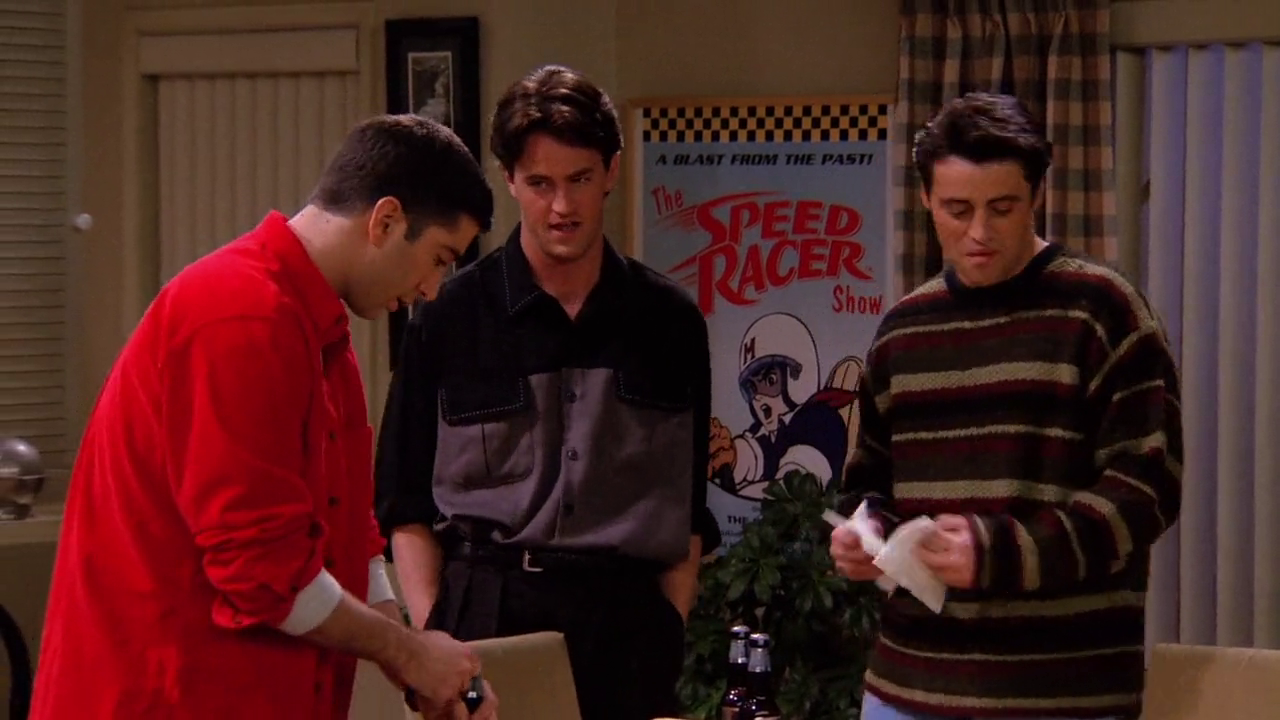
\includegraphics[trim={0 8cm 0 2cm,}, clip, width=\paperwidth]{./S01/img/18/black-bart-speech.png}
    % \caption{Black Bart speech\label{fig:black-bart-speech}}
  \end{adjustwidth}
\end{figure}

\begin{tcolorbox}[enhanced,center upper,
    drop fuzzy shadow southeast, boxrule=0.3pt,
    lower separated=false, breakable,
    colframe=black!30!dialogoBorder,colback=white]
\begin{minipage}[c]{0.16\linewidth}
  \raisebox{\dimexpr-\height+\ht\strutbox\relax}{
    \centering 
\includegraphics[width=1.4cm]{./assets/img/chandler.png}
  }
   & \centering \scriptsize{Chandler}
\end{minipage}
\hfill
\begin{minipage}[c]{0.8\linewidth}
  \textbf{- What was with that whole Black Bart speech? "When I play poker, I'm not a nice guy".}\\
  - E aquele discurso de Black Bart? "Quando jogo pôquer, não sou bonzinho!"
\end{minipage}
\end{tcolorbox}

Ainda na intenção de fazer Ross admitir que está apaixonado por Rachel,
Chandler compara a maneira de falar de Ross com a de \emph{Black Bart},
personagem principal do filme \emph{Blazing Saddles} (1974), uma comédia
de faroeste estadunidense.

\hypertarget{referuxeancias-6}{%
\subsection{Referências}\label{referuxeancias-6}}

\begin{itemize}
\tightlist
\item
  \sloppy Connections - IMDB. \url{https://www.imdb.com/title/tt0583510/movieconnections}
\end{itemize}

\hypertarget{the-lion-sleeps-tonight}{%
\section{The Lion Sleeps Tonight}\label{the-lion-sleeps-tonight}}

\begin{figure}[!ht]
  \begin{adjustwidth}{-\oddsidemargin-1in}{-\rightmargin}
    \centering
    
\includegraphics[trim={0 7cm 0 3cm,}, clip, width=\paperwidth]{./S01/img/18/the-lion-sleeps-tonight.png}
    % \caption{The Lion Sleeps Tonight\label{fig:the-lion-sleeps-tonight}}
  \end{adjustwidth}
\end{figure}

Enquanto os rapazes discutem se Ross ainda sente algo por Rachel, Marcel
aproveita para colocar um CD com a música \emph{The Lion Sleeps Tonight}
(1961), uma versão criada pela banda \emph{The Tokens} (1955). A canção
original chama-se \emph{Mbube} e foi gravada em 1939 pelo cantor
sul-africano \emph{Solomon Linda} (1909-1962) e sua banda \emph{Evening
Birds}.

A música ficou conhecida por estar na trilha sonora do filme \emph{The
Lion King} (1994), no Brasil \emph{O Rei Leão}, filme produzido pela
\emph{Walt Disney}. Ela voltará a ser citada no episódio
\textbf{\textcolor{primarycolor}{S02E12 - Aquele depois do Super Bowl: Parte 1}},
quando os amigos reencontram Marcel no \emph{set} de filmagem.

\hypertarget{referuxeancias-7}{%
\subsection{Referências}\label{referuxeancias-7}}

\begin{itemize}
\tightlist
\item
  \sloppy Revista Rolling Stones (Inglês). \url{https://www.rollingstone.com/music/music-features/lion-sleeps-tonight-lion-king-update-879663/}
\item
  \sloppy The Tokens - Last.fm. \url{https://www.last.fm/music/The+Tokens/+wiki}
\end{itemize}

\hypertarget{kettle-youre-black}{%
\section{Kettle, you're black}\label{kettle-youre-black}}

\begin{figure}[!ht]
  \begin{adjustwidth}{-\oddsidemargin-1in}{-\rightmargin}
    \centering
    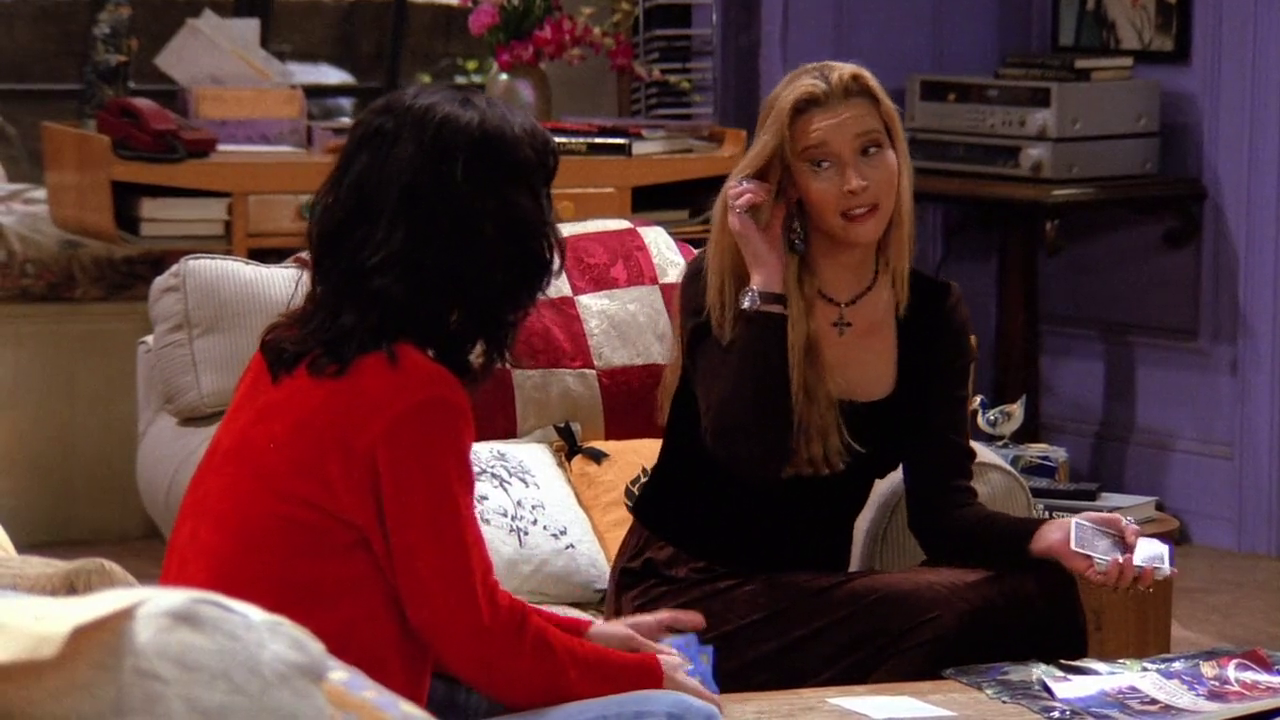
\includegraphics[trim={0 6cm 0 2cm,}, clip, width=\paperwidth]{./S01/img/18/kettle-you-re-black.png}
    % \caption{Kettle, you’re black\label{fig:kettle-you-re-black}}
  \end{adjustwidth}
\end{figure}

\begin{tcolorbox}[enhanced,center upper,
    drop fuzzy shadow southeast, boxrule=0.3pt,
    lower separated=false, breakable,
    colframe=black!30!dialogoBorder,colback=white]
\begin{minipage}[c]{0.16\linewidth}
  \raisebox{\dimexpr-\height+\ht\strutbox\relax}{
    \centering 
\includegraphics[width=1.4cm]{./assets/img/monica.png}
  }
   & \centering \scriptsize{Monica}
\end{minipage}
\hfill
\begin{minipage}[c]{0.8\linewidth}
  \textbf{- Yeah, I know. He can get really competitive. What?}\\
  - É, eu sei. Ele pode ser muito competitivo. Quê?
\end{minipage}

\medskip
\begin{minipage}[c]{0.16\linewidth}
  \raisebox{\dimexpr-\height+\ht\strutbox\relax}{
    \centering 
\includegraphics[width=1.4cm]{./assets/img/phoebe.png}
  }
   & \centering \scriptsize{Phoebe}
\end{minipage}
\hfill
\begin{minipage}[c]{0.8\linewidth}
  \textbf{- Oh. 'Hello, Kettle, this is Monica. You're black.'}\\
  - Oh. 'Olá, Chaleira, é a Monica. Você tá preta.'
\end{minipage}
\end{tcolorbox}

As garotas discutem sobre o quão competitivo Ross é. Phoebe utiliza a
expressão idiomática \emph{The pot calling the kettle black}. Em
português, uma expressão com o mesmo significado seria \emph{O sujo
falando do mal lavado}, indicando a hipocrisia ao criticar uma outra
pessoa por um defeito que você também possui.

A expressão em Inglês vêm do fato de que os utensílios culinários eram
utilizados sobre chama de fogueiras, que, devido a fumaça, deixam
panelas e chaleiras com manchas pretas.

\hypertarget{referuxeancias-8}{%
\subsection{Referências}\label{referuxeancias-8}}

\begin{itemize}
\tightlist
\item
  \sloppy Cambridge Dictionary (Inglês). \url{https://dictionary.cambridge.org/pt/dicionario/ingles/pot-calling-the-kettle-black}
\end{itemize}

\hypertarget{pictionary}{%
\section{Pictionary}\label{pictionary}}

\begin{figure}[!ht]
  \begin{adjustwidth}{-\oddsidemargin-1in}{-\rightmargin}
    \centering
    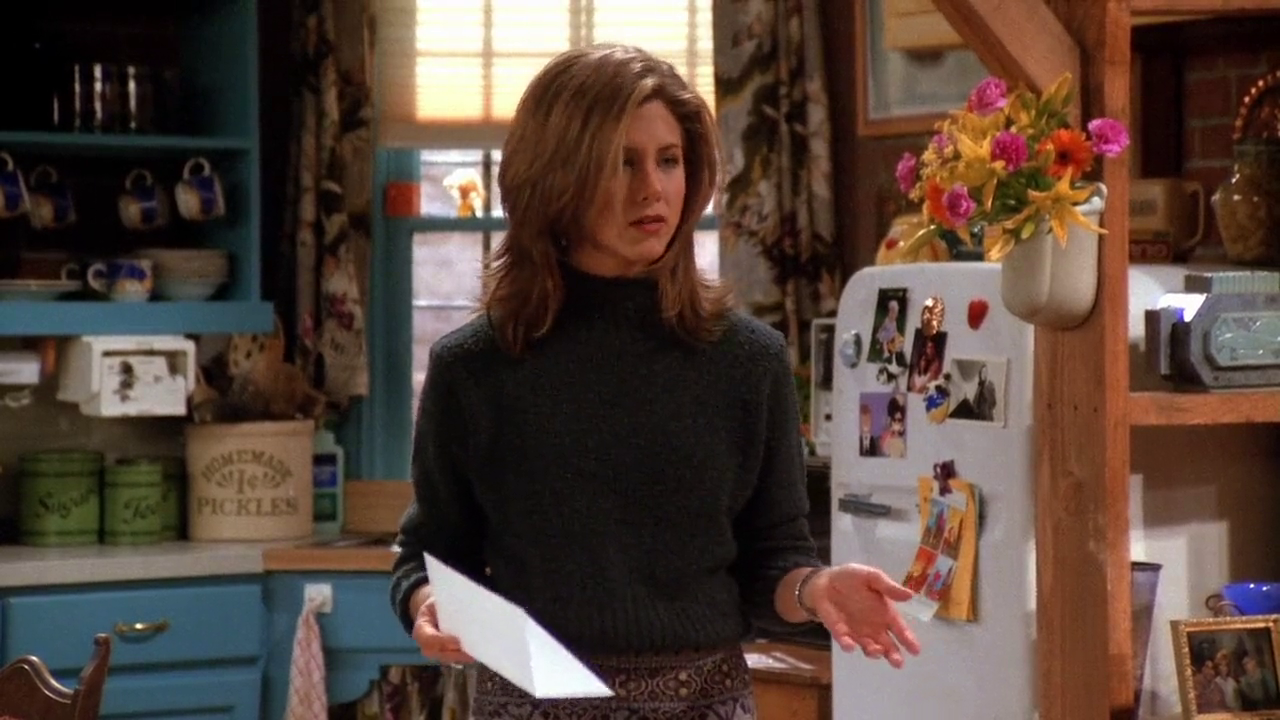
\includegraphics[trim={0 6cm 0 2cm,}, clip, width=\paperwidth]{./S01/img/18/pictionary.png}
    % \caption{Pictionary\label{fig:pictionary}}
  \end{adjustwidth}
\end{figure}

\begin{tcolorbox}[enhanced,center upper,
    drop fuzzy shadow southeast, boxrule=0.3pt,
    lower separated=false, breakable,
    colframe=black!30!dialogoBorder,colback=white]
\begin{minipage}[c]{0.16\linewidth}
  \raisebox{\dimexpr-\height+\ht\strutbox\relax}{
    \centering 
\includegraphics[width=1.4cm]{./assets/img/rachel.png}
  }
   & \centering \scriptsize{Rachel}
\end{minipage}
\hfill
\begin{minipage}[c]{0.8\linewidth}
  \textbf{- Oh, I beg to differ. The Pictionary incident?}\\
  - Tenho que discordar. O incidente com o Imagem e Ação?
\end{minipage}
\end{tcolorbox}

Monica tenta escapar da pecha de ser tão competitiva quanto Ross, mas
Rachel lembra do incidente com o jogo \emph{Pictionary} (1985), onde
ela, aparentemente sem querer, arremessou um prato na direção de sua
equipe. Ao final do episódio os amigos acabam jogando uma partida e o
jogo deve ser jogado por equipes onde um membro da equipe precisa
desenhar e os outros precisam adivinhar do que se trata o desenho. Além
de adivinhar, é preciso percorrer um tabuleiro que irá ajudar a
selecionar que tipo de palavra pode ser escolhida, seja uma pessoa, um
lugar, um objeto, uma ação, um filme, etc.

No Brasil o jogo foi adaptado pela \emph{Grow} com o nome de
\emph{Imagem \& Ação}.

\hypertarget{referuxeancias-9}{%
\subsection{Referências}\label{referuxeancias-9}}

\begin{itemize}
\tightlist
\item
  \sloppy Site oficial (Inglês). \url{https://www.mattelgames.com/en-us/family/pictionary}
\item
  \sloppy Fandom Wiki (Inglês). \url{https://pictionary.fandom.com/wiki/Pictionary}
\item
  \sloppy Imagem \& Ação - Metropoly. \url{https://www.metropolybar.com.br/imagem-e-acao-um-sucesso-na-vida-real-na-tv-e-nos-games/}
\end{itemize}

\hypertarget{saks-fifth-avenue}{%
\section{Saks Fifth Avenue}\label{saks-fifth-avenue}}

\begin{figure}[!ht]
  \begin{adjustwidth}{-\oddsidemargin-1in}{-\rightmargin}
    \centering
    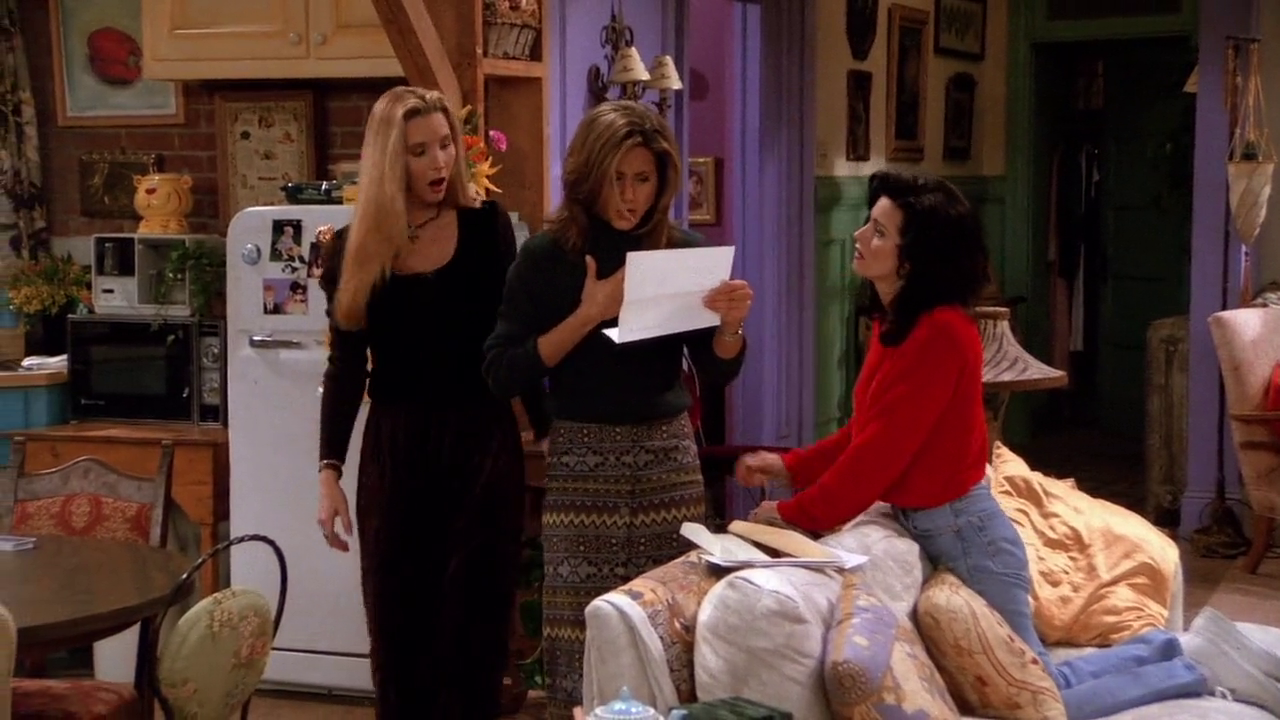
\includegraphics[trim={0 6cm 0 2cm,}, clip, width=\paperwidth]{./S01/img/18/saks-fifth-avenue.png}
    % \caption{Saks Fifth Avenue\label{fig:saks-fifth-avenue}}
  \end{adjustwidth}
\end{figure}

\begin{tcolorbox}[enhanced,center upper,
    drop fuzzy shadow southeast, boxrule=0.3pt,
    lower separated=false, breakable,
    colframe=black!30!dialogoBorder,colback=white]
\begin{minipage}[c]{0.16\linewidth}
  \raisebox{\dimexpr-\height+\ht\strutbox\relax}{
    \centering 
\includegraphics[width=1.4cm]{./assets/img/rachel.png}
  }
   & \centering \scriptsize{Rachel}
\end{minipage}
\hfill
\begin{minipage}[c]{0.8\linewidth}
  \textbf{- I got an interview. I got an interview.}\\
  - Tenho uma entrevista. Tenho uma entrevista.
\end{minipage}

\medskip
\begin{minipage}[c]{0.16\linewidth}
  \raisebox{\dimexpr-\height+\ht\strutbox\relax}{
    \centering 
\includegraphics[width=1.4cm]{./assets/img/monica.png}
  }
   & \centering \scriptsize{Monica}
\end{minipage}
\hfill
\begin{minipage}[c]{0.8\linewidth}
  \textbf{- You're kidding. Where? Where?}\\
  - Tá brincando. Onde? Onde?
\end{minipage}

\medskip
\begin{minipage}[c]{0.16\linewidth}
  \raisebox{\dimexpr-\height+\ht\strutbox\relax}{
    \centering 
\includegraphics[width=1.4cm]{./assets/img/rachel.png}
  }
   & \centering \scriptsize{Rachel}
\end{minipage}
\hfill
\begin{minipage}[c]{0.8\linewidth}
  \textbf{- Saks Fifth Avenue.}\\
  - Saks Fifth Avenue.
\end{minipage}

\medskip
\begin{minipage}[c]{0.16\linewidth}
  \raisebox{\dimexpr-\height+\ht\strutbox\relax}{
    \centering 
\includegraphics[width=1.4cm]{./assets/img/phoebe.png}
  }
   & \centering \scriptsize{Phoebe}
\end{minipage}
\hfill
\begin{minipage}[c]{0.8\linewidth}
  \textbf{- Oh, it's like the mother ship is calling you home.}\\
  - É como se a nave-mãe a chamasse para voltar.
\end{minipage}
\end{tcolorbox}

Rachel recebe uma carta informando que ela foi selecionada para uma
entrevista na \emph{Saks Fifth Avenue} (1924), uma cadeia americana de
lojas de departamento de luxo. Seu nome vem do fato de sua localização,
a famosa \emph{Fifth Avenue}, ou \emph{Quinta Avenida}, situada em
\emph{Manhattan - NY}.

\hypertarget{referuxeancias-10}{%
\subsection{Referências}\label{referuxeancias-10}}

\begin{itemize}
\tightlist
\item
  \sloppy Site oficial (Inglês). \url{https://www.saksfifthavenue.com/main/static_content.jsp?pageId=about-us}
\end{itemize}

\hypertarget{tony-randall}{%
\section{Tony Randall}\label{tony-randall}}

\begin{figure}[!ht]
  \begin{adjustwidth}{-\oddsidemargin-1in}{-\rightmargin}
    \centering
    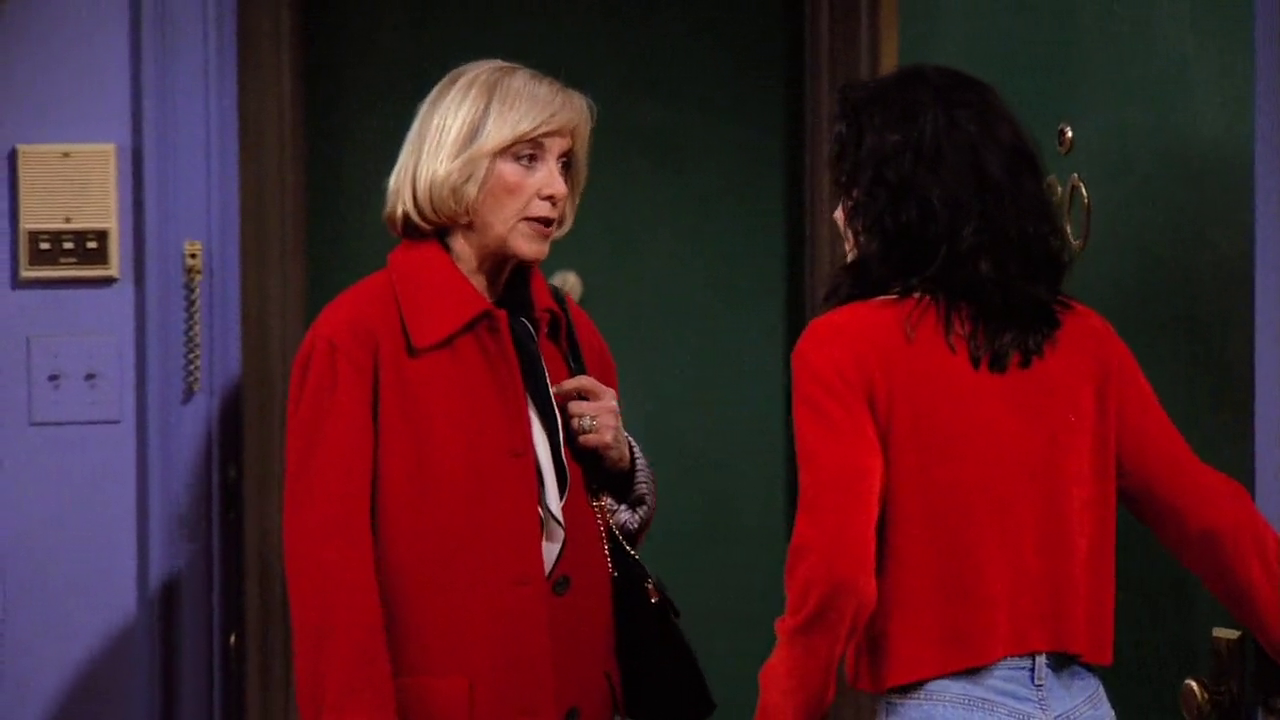
\includegraphics[trim={0 8cm 0 2cm,}, clip, width=\paperwidth]{./S01/img/18/tony-randall.png}
    % \caption{Tony Randall\label{fig:tony-randall}}
  \end{adjustwidth}
\end{figure}

\begin{tcolorbox}[enhanced,center upper,
    drop fuzzy shadow southeast, boxrule=0.3pt,
    lower separated=false, breakable,
    colframe=black!30!dialogoBorder,colback=white]
\begin{minipage}[c]{0.16\linewidth}
  \raisebox{\dimexpr-\height+\ht\strutbox\relax}{
    \centering 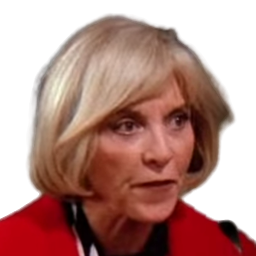
\includegraphics[width=1.4cm]{./assets/img/iris.png}
  }
   & \centering \scriptsize{Iris}
\end{minipage}
\hfill
\begin{minipage}[c]{0.8\linewidth}
  \textbf{- Is Tony Randall dead?}\\
  - Tony Randall morreu?
\end{minipage}

\medskip
\begin{minipage}[c]{0.16\linewidth}
  \raisebox{\dimexpr-\height+\ht\strutbox\relax}{
    \centering 
\includegraphics[width=1.4cm]{./assets/img/monica.png}
  }
   & \centering \scriptsize{Monica}
\end{minipage}
\hfill
\begin{minipage}[c]{0.8\linewidth}
  \textbf{- I don't think so.}\\
  - Acho que não.
\end{minipage}

\medskip
\begin{minipage}[c]{0.16\linewidth}
  \raisebox{\dimexpr-\height+\ht\strutbox\relax}{
    \centering 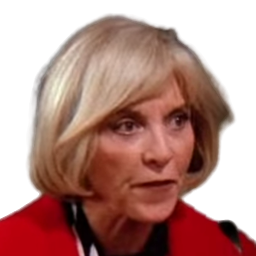
\includegraphics[width=1.4cm]{./assets/img/iris.png}
  }
   & \centering \scriptsize{Iris}
\end{minipage}
\hfill
\begin{minipage}[c]{0.8\linewidth}
  \textbf{- Well, he may be now because I think I hit him with my car.}\\
  - Bem, pode ser que sim porque acho que o atropelei.
\end{minipage}

\medskip
\begin{minipage}[c]{0.16\linewidth}
  \raisebox{\dimexpr-\height+\ht\strutbox\relax}{
    \centering 
\includegraphics[width=1.4cm]{./assets/img/monica.png}
  }
   & \centering \scriptsize{Monica}
\end{minipage}
\hfill
\begin{minipage}[c]{0.8\linewidth}
  \textbf{- My God. Really?}\\
  - Meu Deus. Sério?
\end{minipage}

\medskip
\begin{minipage}[c]{0.16\linewidth}
  \raisebox{\dimexpr-\height+\ht\strutbox\relax}{
    \centering 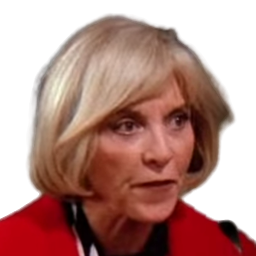
\includegraphics[width=1.4cm]{./assets/img/iris.png}
  }
   & \centering \scriptsize{Iris}
\end{minipage}
\hfill
\begin{minipage}[c]{0.8\linewidth}
  \textbf{- No, that's bluffing. Lesson number one.}\\
  - Não, foi um blefe. Lição número um.
\end{minipage}
\end{tcolorbox}

A fim de uma revanche contra os rapazes, as moças se encontram com a Tia
Iris - a qual joga poker desde os cinco anos de idade-, que logo que
chega tenta ensinar o blefe, informando que atropelou \emph{Tony
Randall} (1920-2004), ator americano conhecido por seu trabalho em
\emph{The Odd Couple}, \emph{sitcom} já citada em
\textbf{\textcolor{primarycolor}{S01E12 - Aquele com uma Dúzia de Lasanhas}}.

\begin{figure}
  \centering
  \begin{tikzpicture}
    \node [inner sep=0pt] at (0,0) {
      
\includegraphics[width=0.8\textwidth,keepaspectratio]{./S01/img/18/tony-randall-odd-couple.png}
    };
    \draw [white, rounded corners=\ClipSep, line width=\ClipSep]
    (current bounding box.north west) --
    (current bounding box.north east) --
    (current bounding box.south east) --
    (current bounding box.south west) -- cycle
    ;
    \end{tikzpicture}
    \caption{Tony Randall e Jack Klugman - Odd Couple\label{fig:tony-randall-e-jack-klugman-odd-couple}}
\end{figure}

\emph{Tony Randall} (à esquerda) ao lado de \emph{Jack Klugman}.

\hypertarget{referuxeancias-11}{%
\subsection{Referências}\label{referuxeancias-11}}

\begin{itemize}
\tightlist
\item
  \sloppy Tony Randall - Encyclopædia Britannica. \url{https://www.britannica.com/biography/Tony-Randall}
\end{itemize}

\hypertarget{to-build-you-need-to-know-to-know-you-have-to-learn}{%
\section{To build you need to know, to know you have to
learn}\label{to-build-you-need-to-know-to-know-you-have-to-learn}}

\begin{figure}[!ht]
  \begin{adjustwidth}{-\oddsidemargin-1in}{-\rightmargin}
    \centering
    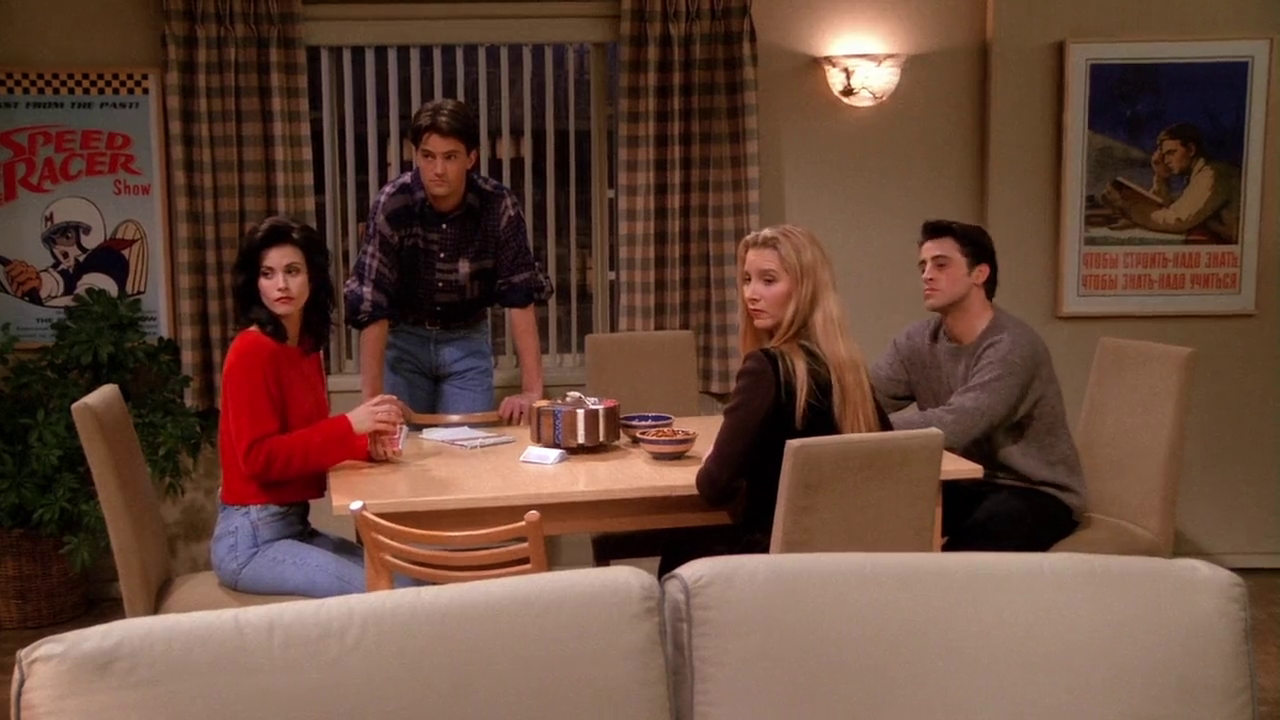
\includegraphics[trim={0 7cm 0 2cm,}, clip, width=\paperwidth]{./S01/img/18/to-build-you-need-to-know.png}
    % \caption{To build you need to know, to know you have to learn\label{fig:to-build-you-need-to-know-to-know-you-have-to-learn}}
  \end{adjustwidth}
\end{figure}

Mais uma vez na sala do Ross, é possível ver um poster soviético com a
frase em russo, que traduzindo para o Inglês seria \emph{To build you
need to know, to know you have to learn} (1958), que quer dizer
\emph{Para construir é preciso conhecimento, para ter conhecimento é
preciso aprendizado}.

\begin{figure}
  \centering
  \begin{tikzpicture}
    \node [inner sep=0pt] at (0,0) {
      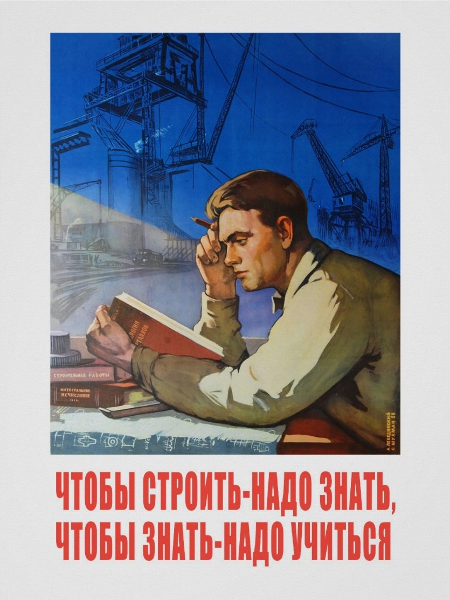
\includegraphics[width=0.6\textwidth,keepaspectratio]{./S01/img/18/to-build-you-need-to-know-poster.jpg}
    };
    \draw [white, rounded corners=\ClipSep, line width=\ClipSep]
    (current bounding box.north west) --
    (current bounding box.north east) --
    (current bounding box.south east) --
    (current bounding box.south west) -- cycle
    ;
    \end{tikzpicture}
    \caption{To build you need to know, to know you have to learn - Poster\label{fig:to-build-you-need-to-know-to-know-you-have-to-learn-poster}}
\end{figure}

\hypertarget{referuxeancias-12}{%
\subsection{Referências}\label{referuxeancias-12}}

\begin{itemize}
\tightlist
\item
  \sloppy The One with the Illustrated Posters (Inglês). \url{https://illustrationchronicles.com/The-One-with-the-Illustrated-Posters}
\end{itemize}

\hypertarget{trident}{%
\section{Trident}\label{trident}}

\begin{figure}[!ht]
  \begin{adjustwidth}{-\oddsidemargin-1in}{-\rightmargin}
    \centering
    
\includegraphics[trim={0 7cm 0 1cm,}, clip, width=\paperwidth]{./S01/img/18/trident.png}
    % \caption{Trident\label{fig:trident}}
  \end{adjustwidth}
\end{figure}

\begin{tcolorbox}[enhanced,center upper,
    drop fuzzy shadow southeast, boxrule=0.3pt,
    lower separated=false, breakable,
    colframe=black!30!dialogoBorder,colback=white]
\begin{minipage}[c]{0.16\linewidth}
  \raisebox{\dimexpr-\height+\ht\strutbox\relax}{
    \centering 
\includegraphics[width=1.4cm]{./assets/img/rachel.png}
  }
   & \centering \scriptsize{Rachel}
\end{minipage}
\hfill
\begin{minipage}[c]{0.8\linewidth}
  \textbf{- Guess what, guess what, guess what.}\\
  - Adivinhem, adivinhem.
\end{minipage}

\medskip
\begin{minipage}[c]{0.16\linewidth}
  \raisebox{\dimexpr-\height+\ht\strutbox\relax}{
    \centering 
\includegraphics[width=1.4cm]{./assets/img/chandler.png}
  }
   & \centering \scriptsize{Chandler}
\end{minipage}
\hfill
\begin{minipage}[c]{0.8\linewidth}
  \textbf{- Uh, okay. The fifth dentist caved, and now they're all recommending Trident?}\\
  - Ah, sim. O quinto dentista cedeu, e agora todos recomendam Trident?
\end{minipage}
\end{tcolorbox}

Rachel tenta dar boas notícias em relação a sua entrevista mas Chandler,
sarcástico como sempre, faz referência a goma de mascar (lembre-se que
\emph{chiclete} é uma marca) \emph{Trident} (1964) e seu famoso
comercial que dizia \emph{``Four out of five dentists surveyed recommend
sugarless gums for their patients who chew gum''}, traduzindo
\emph{``Quatro de cada cinco dentistas recomendam goma sem açúcar para
pacientes que mascam goma''}.

Essa referência remete ao episódio
\textbf{\textcolor{primarycolor}{S01E07 - Aquele com o Blecaute}}, em
que Chandler não aceita goma de mascar de \emph{Jill Goodacre}, por que
não era dietética.

\hypertarget{referuxeancias-13}{%
\subsection{Referências}\label{referuxeancias-13}}

\begin{itemize}
\tightlist
\item
  \sloppy NY Times (Inglês). \url{https://www.nytimes.com/2009/07/28/business/media/28adco.html}
\item
  \sloppy Comercial de 1977 - YouTube. \url{https://www.youtube.com/watch?v=YWtvytMgQB8}
\end{itemize}

\hypertarget{airport}{%
\section{Airport}\label{airport}}

\begin{figure}[!ht]
  \begin{adjustwidth}{-\oddsidemargin-1in}{-\rightmargin}
    \centering
    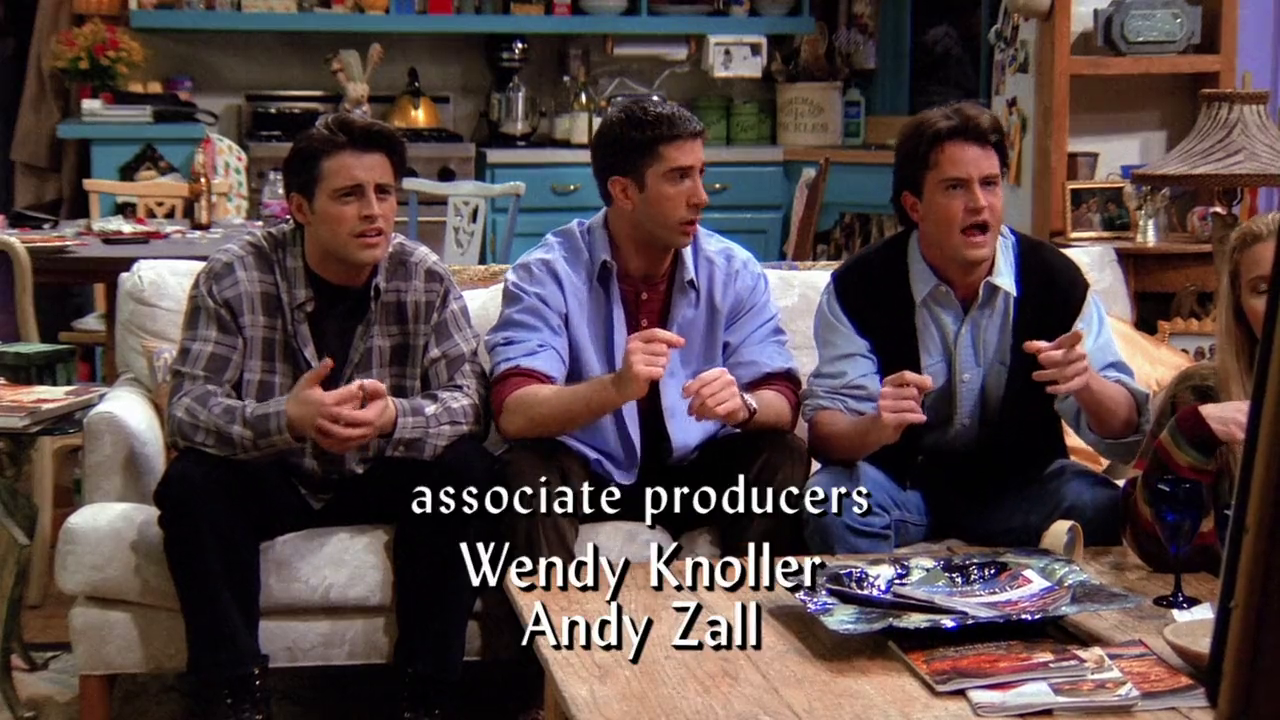
\includegraphics[trim={0 7cm 0 2cm,}, clip, width=\paperwidth]{./S01/img/18/airport.png}
    % \caption{Airport\label{fig:airport}}
  \end{adjustwidth}
\end{figure}

\begin{tcolorbox}[enhanced,center upper,
    drop fuzzy shadow southeast, boxrule=0.3pt,
    lower separated=false, breakable,
    colframe=black!30!dialogoBorder,colback=white]
\begin{minipage}[c]{0.16\linewidth}
  \raisebox{\dimexpr-\height+\ht\strutbox\relax}{
    \centering 
\includegraphics[width=1.4cm]{./assets/img/chandler.png}
  }
   & \centering \scriptsize{Chandler}
\end{minipage}
\hfill
\begin{minipage}[c]{0.8\linewidth}
  \textbf{- Airplane! Airport! Airport '75! Airport '77! Airport '79!}\\
  - Airplane! Airport! Airport '75! Airport '77! Airport '79!
\end{minipage}
\end{tcolorbox}

Na tentativa de adivinhar o desenho de Monica, Chandler faz referência a
série de filmes: \emph{Airport} (1970), \emph{Airport '75} (1974),
\emph{Airport '77} (1977) e \emph{Airport '79} (1979). Todos tem a mesma
premissa de um filme de drama e suspense que envolve um acidente com um
avião. Ele ainda chuta \emph{Airplane!} (1980), uma comédia satírica
americana, que também envolve uma catástrofe aérea mas de forma cômica.

No Brasil os filmes são conhecidos como \emph{Aeroporto},
\emph{Aeroporto 75}, \emph{Aeroporto 77}, \emph{Aeroporto 79: O
Concorde} e \emph{Apertem os Cintos, o Piloto Sumiu}, respectivamente.

\hypertarget{referuxeancias-14}{%
\subsection{Referências}\label{referuxeancias-14}}

\begin{itemize}
\tightlist
\item
  \sloppy Airport - IMDB. \url{https://www.imdb.com/title/tt0065377/}
\item
  \sloppy Airport ’75 - IMDB. \url{https://www.imdb.com/title/tt0071110/?ref_=tt_sims_tt}
\item
  \sloppy Airport ’77 - IMDB. \url{https://www.imdb.com/title/tt0075648/?ref_=tt_sims_tt}
\item
  \sloppy Airport ’79 - IMDB. \url{https://www.imdb.com/title/tt0078740/?ref_=tt_sims_tt}
\item
  \sloppy Airplane! - IMDB. \url{https://www.imdb.com/title/tt0080339/}
\end{itemize}

\hypertarget{bye-bye-birdie}{%
\section{Bye Bye Birdie}\label{bye-bye-birdie}}

\begin{figure}[!ht]
  \begin{adjustwidth}{-\oddsidemargin-1in}{-\rightmargin}
    \centering
    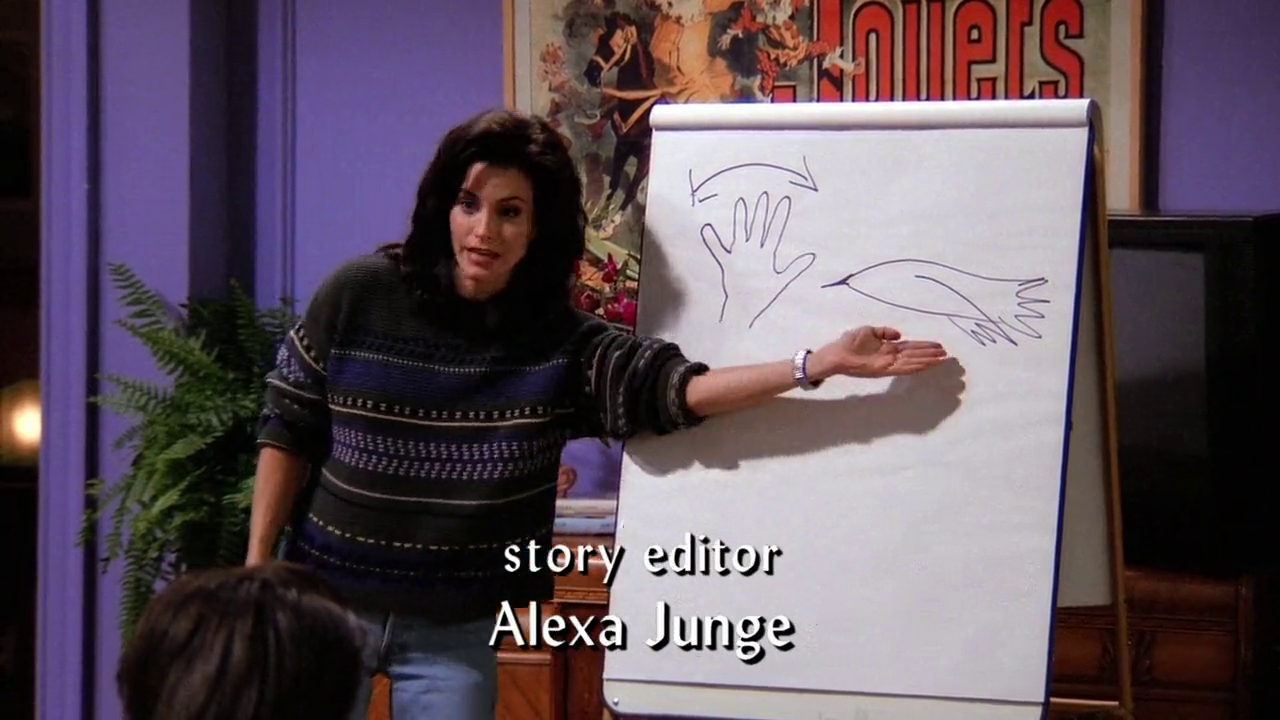
\includegraphics[trim={0 7cm 0 2cm,}, clip, width=\paperwidth]{./S01/img/18/bye-bye-birdie.png}
    % \caption{Bye Bye Birdie\label{fig:bye-bye-birdie}}
  \end{adjustwidth}
\end{figure}

\begin{tcolorbox}[enhanced,center upper,
    drop fuzzy shadow southeast, boxrule=0.3pt,
    lower separated=false, breakable,
    colframe=black!30!dialogoBorder,colback=white]
\begin{minipage}[c]{0.16\linewidth}
  \raisebox{\dimexpr-\height+\ht\strutbox\relax}{
    \centering 
\includegraphics[width=1.4cm]{./assets/img/monica.png}
  }
   & \centering \scriptsize{Monica}
\end{minipage}
\hfill
\begin{minipage}[c]{0.8\linewidth}
  \textbf{- Bye Bye Birdie.}\\
  - Bye Bye Birdie.
\end{minipage}

\medskip
\begin{minipage}[c]{0.16\linewidth}
  \raisebox{\dimexpr-\height+\ht\strutbox\relax}{
    \centering \includegraphics[width=1.4cm]{./assets/img/phoebe.png}
  }
   & \centering \scriptsize{Phoebe}
\end{minipage}
\hfill
\begin{minipage}[c]{0.8\linewidth}
  \textbf{- That's a bird? That's a bird.}\\
  - Isso é um pássaro? Isso é um pássaro.
\end{minipage}
\end{tcolorbox}

Monica tenta fazer um desenho para sua equipe adivinhar o filme
\emph{Bye Bye Birdie} (1963), que conta a história de um cantor de
\emph{rock} no auge da carreira que foi convocado a servir no exército,
que é baseado na história de \emph{Elvis Presley} (1935-1977). No Brasil
o filme se chama \emph{Adeus, Amor}.

\begin{figure}
  \centering
  \begin{tikzpicture}
    \node [inner sep=0pt] at (0,0) {
      \includegraphics[width=0.6\textwidth,keepaspectratio]{./S01/img/18/bye-bye-birdie-poster.jpg}
    };
    \draw [white, rounded corners=\ClipSep, line width=\ClipSep]
    (current bounding box.north west) --
    (current bounding box.north east) --
    (current bounding box.south east) --
    (current bounding box.south west) -- cycle
    ;
    \end{tikzpicture}
    \caption{Bye Bye Birdie - Poster\label{fig:bye-bye-birdie-poster}}
\end{figure}

\hypertarget{referuxeancias-15}{%
\subsection{Referências}\label{referuxeancias-15}}

\begin{itemize}
\tightlist
\item
  \sloppy IMDB. \url{https://www.imdb.com/title/tt0056891/}
\end{itemize}

\hypertarget{the-unbearable-lightness-of-being}{%
\section{The Unbearable Lightness of
Being}\label{the-unbearable-lightness-of-being}}

\begin{figure}[!ht]
  \begin{adjustwidth}{-\oddsidemargin-1in}{-\rightmargin}
    \centering
    \includegraphics[trim={0 7cm 0 2cm,}, clip, width=\paperwidth]{./S01/img/18/the-unbearable-lightness-of-being.png}
    % \caption{The Unbearable Lightness of Being\label{fig:the-unbearable-lightness-of-being}}
  \end{adjustwidth}
\end{figure}

\begin{tcolorbox}[enhanced,center upper,
    drop fuzzy shadow southeast, boxrule=0.3pt,
    lower separated=false, breakable,
    colframe=black!30!dialogoBorder,colback=white]
\begin{minipage}[c]{0.16\linewidth}
  \raisebox{\dimexpr-\height+\ht\strutbox\relax}{
    \centering \includegraphics[width=1.4cm]{./assets/img/rachel.png}
  }
   & \centering \scriptsize{Rachel}
\end{minipage}
\hfill
\begin{minipage}[c]{0.8\linewidth}
  \textbf{- Okay, okay, it's my turn.}\\
  - Tá bom. Minha vez.
\end{minipage}

\medskip
\begin{minipage}[c]{0.16\linewidth}
  \raisebox{\dimexpr-\height+\ht\strutbox\relax}{
    \centering \includegraphics[width=1.4cm]{./assets/img/ross.png}
  }
   & \centering \scriptsize{Ross}
\end{minipage}
\hfill
\begin{minipage}[c]{0.8\linewidth}
  \textbf{- Bean. Bean.}\\
  - Cevada. Ce...
\end{minipage}

\medskip
\begin{minipage}[c]{0.16\linewidth}
  \raisebox{\dimexpr-\height+\ht\strutbox\relax}{
    \centering \includegraphics[width=1.4cm]{./assets/img/joey.png}
  }
   & \centering \scriptsize{Joey}
\end{minipage}
\hfill
\begin{minipage}[c]{0.8\linewidth}
  \textbf{- The Unbearable Lightness of Being.}\\
  - A Insustentável Leveza do Ser.
\end{minipage}
\end{tcolorbox}

Na vez da Rachel ela desenha um feijão, que em Inglês pode ser traduzido
como \emph{bean}, e que tem pronúncia semelhante à de \emph{being}. Daí
que Joey acerta com o filme \emph{The Unbearable Lightness of Being}
(1988), drama que conta a história de um médico Checo com uma vida
sexual ativa que conhece uma mulher que quer monogamia, e a invasão
Soviética em 1968 atrapalha ainda mais suas vidas.

É o tipo de piada que, geralmente, só funciona no país de origem, ou
onde as línguas são parecidas. A cena ainda envolve um desenho que torna
a tradução mais complicada, já que há um elemento visual que restringe
uma melhor adaptação.

\begin{figure}
  \centering
  \begin{tikzpicture}
    \node [inner sep=0pt] at (0,0) {
      \includegraphics[width=0.6\textwidth,keepaspectratio]{./S01/img/18/the-unbearable-lightness-of-being-poster.jpg}
    };
    \draw [white, rounded corners=\ClipSep, line width=\ClipSep]
    (current bounding box.north west) --
    (current bounding box.north east) --
    (current bounding box.south east) --
    (current bounding box.south west) -- cycle
    ;
    \end{tikzpicture}
    \caption{The Unbearable Lightness of Being - Poster\label{fig:the-unbearable-lightness-of-being-poster}}
\end{figure}

\hypertarget{referuxeancias-16}{%
\subsection{Referências}\label{referuxeancias-16}}

\begin{itemize}
\tightlist
\item
  \sloppy IMDB. \url{https://www.imdb.com/title/tt0096332/?ref_=nv_sr_srsg_0}
\end{itemize}
